\documentclass[11pt]{article}
\usepackage[utf8]{inputenc}
\usepackage[T1]{fontenc}
\usepackage{geometry}
\usepackage{enumitem}
\usepackage{hyperref}
\usepackage{amsmath}
\usepackage{booktabs}
\usepackage{array}
\usepackage{tabularx}
\usepackage{graphicx}
\usepackage{float}
\geometry{a4paper, margin=1in}
\graphicspath{{../results/figures/}}

\hypersetup{
    colorlinks=true,
    linkcolor=blue,
    urlcolor=cyan,
    citecolor=blue
}

\title{\textbf{k-Anonymity-Based Data Anonymization and Re-identification Risk Analysis}\\
\large MSCS 714 Data Privacy Seminar}
\author{Group Project}
\date{April 2026}

\begin{document}

\maketitle

\begin{abstract}
This report presents an implementation and evaluation of k-anonymity on the Adult Census Income dataset. The project compares two quasi-identifier sets, two anonymization strategies, and three privacy levels ($k=2,5,10$), resulting in 12 experiment settings. The pipeline uses only generalization and suppression, matching the project scope exactly. Linkage risk is evaluated with exact-match attacks using five independently sampled auxiliary datasets, and utility is measured through row retention, income-distribution shift, hours-per-week distortion, and a direct information-loss score that captures both suppression and generalization. Across all 12 settings, the exact unique match rate drops to zero. However, the strategies achieve that outcome very differently. The generalization-first strategy preserves all rows but incurs heavy information loss (0.67 to 0.92), while the improved targeted-suppression strategy combines mild generalization with selective removal and retains 94.0\% to 98.7\% of the data. The results show a clearer and more realistic privacy--utility trade-off than the initial baseline: stronger privacy increases attack failure, but it also increases information loss. The best overall balance in this implementation is achieved by targeted suppression with low $k$, especially QI Set A at $k=2$.
\end{abstract}

\section{Introduction}
Removing names from a dataset does not make it automatically private. In many real data releases, individuals can still be re-identified by linking \textit{quasi-identifiers} such as age, sex, education, occupation, or location with external information. This is the central linkage-attack problem in data privacy.

This project studies that problem through \textbf{k-anonymity}. A release satisfies k-anonymity when every visible quasi-identifier combination appears in at least $k$ records. In theory, this should prevent exact unique linkage on those attributes. In practice, however, stronger privacy often requires more aggressive generalization or suppression, reducing the value of the released data.

The goal of the project is therefore not only to enforce k-anonymity, but also to evaluate the privacy--utility trade-off created by different anonymization choices. The final system and report stay within the exact scope of Project 4: no l-diversity, no differential privacy, and no cryptography.

\section{Problem Statement and Objectives}
The project investigates the following question:

\begin{quote}
How do different values of $k$, different quasi-identifier choices, and different anonymization strategies affect exact-match linkage risk and analytical utility in the Adult Census Income dataset?
\end{quote}

The main objectives are:
\begin{itemize}[leftmargin=*]
    \item build a reproducible Python pipeline for k-anonymization;
    \item evaluate $k=2$, $k=5$, and $k=10$;
    \item compare two quasi-identifier (QI) sets;
    \item compare a generalization-first strategy with a more balanced targeted-suppression strategy;
    \item simulate linkage attacks using auxiliary data;
    \item measure both attack outcomes and utility degradation with interpretable metrics.
\end{itemize}

\section{Related Work}
k-anonymity was formalized by Samarati and Sweeney and later developed by Sweeney as a practical model for limiting re-identification in released data \cite{SamaratiSweeney1998,Sweeney2002}. Their work established the core intuition behind this project: combinations of demographic attributes can identify individuals even after direct identifiers are removed.

Bayardo and Agrawal examined optimal k-anonymization under generalization and suppression, showing that privacy protection and utility preservation must be balanced carefully \cite{BayardoAgrawal2005}. Their work motivates the heuristic search-based implementation used here rather than an expensive optimization procedure.

Later work on \textit{l-diversity} and \textit{t-closeness} demonstrated that k-anonymity alone does not eliminate every privacy risk, especially when sensitive values remain homogeneous inside equivalence classes \cite{Machanavajjhala2007,Li2007}. Those extensions are outside this project's scope, but they help position its limitations.

Fung et al.\ provide a broader survey of privacy-preserving data publishing methods and their trade-offs \cite{Fung2010}. The Adult dataset remains a widely used benchmark because of its realistic mixture of continuous and categorical demographic attributes \cite{Kohavi1996,UCIAdult}.

\section{Dataset Description}
\subsection{Source and Structure}
The experiments use the \textbf{Adult Census Income} dataset from the UCI Machine Learning Repository. The local file used in this project is stored at \texttt{data/raw/adult/adult.data}. It contains \textbf{32,561} rows and \textbf{15} columns.

\subsection{Observed Dataset Characteristics}
Inspection of the local data produced the following summary:
\begin{itemize}[leftmargin=*]
    \item total rows: 32,561
    \item total columns: 15
    \item age range: 17 to 90, mean 38.58
    \item hours-per-week range: 1 to 99, mean 40.44
    \item income distribution: 24,720 with \texttt{<=50K} and 7,841 with \texttt{>50K}
    \item missing values encoded as \texttt{?}: \texttt{workclass} (1,836), \texttt{occupation} (1,843), \texttt{native-country} (583)
\end{itemize}

\subsection{Attribute Roles}
Table~\ref{tab:attribute_roles} summarizes how the columns were used.

\begin{table}[H]
\centering
\begin{tabularx}{\textwidth}{>{\raggedright\arraybackslash}p{0.24\textwidth} >{\raggedright\arraybackslash}p{0.18\textwidth} X}
\toprule
\textbf{Attribute} & \textbf{Role} & \textbf{Rationale} \\
\midrule
\texttt{income} & Sensitive attribute & Preserved for risk and utility analysis. \\
\texttt{age}, \texttt{sex}, \texttt{education}, \texttt{marital-status} & QI Set A & Moderate-risk demographic combination with stable categorical values. \\
\texttt{age}, \texttt{sex}, \texttt{occupation}, \texttt{native-country} & QI Set B & Sparser, more detailed combination representing a stronger attack scenario. \\
\texttt{hours-per-week}, \texttt{education-num} & Utility attributes & Retained for simple statistical comparisons. \\
\texttt{workclass}, \texttt{relationship}, \texttt{race}, \texttt{capital-gain}, \texttt{capital-loss}, \texttt{fnlwgt} & Supporting attributes & Present in the dataset but not used in the selected QI sets. \\
\bottomrule
\end{tabularx}
\caption{Attribute roles used in the experiments.}
\label{tab:attribute_roles}
\end{table}

\subsection{Baseline Risk Before Anonymization}
Before any transformation, the raw data already exhibits strong linkage risk:
\begin{itemize}[leftmargin=*]
    \item QI Set A creates 4,331 equivalence classes, including 1,724 singleton classes.
    \item QI Set B creates 4,308 equivalence classes, including 2,526 singleton classes.
\end{itemize}

These singleton classes are the basic motivation for anonymization.

\section{Threat Model}
The attacker is assumed to have an auxiliary table containing quasi-identifiers for a subset of individuals and a synthetic \texttt{person\_id}. The attacker does not know the sensitive attribute (\texttt{income}) but can attempt exact matching between the auxiliary data and the released quasi-identifiers.

To make the evaluation more stable than a single random sample, the implementation generates \textbf{five} auxiliary datasets using different random seeds. Each auxiliary dataset contains 20\% of the original records, which corresponds to 6,512 sampled individuals. The reported linkage metrics are averages over those five attack runs.

\section{Methodology}
\subsection{Preprocessing}
The data pipeline:
\begin{itemize}[leftmargin=*]
    \item loads the Adult file with explicit column names,
    \item trims categorical whitespace,
    \item converts \texttt{?} to missing values,
    \item replaces missing QI-related categories with \texttt{Unknown},
    \item adds a synthetic \texttt{person\_id} for evaluation only,
    \item preserves \texttt{income} as both a raw label and a binary indicator.
\end{itemize}

\subsection{Quasi-Identifier Sets}
The project evaluates:
\begin{itemize}[leftmargin=*]
    \item \textbf{QI Set A:} \{\texttt{age}, \texttt{sex}, \texttt{education}, \texttt{marital-status}\}
    \item \textbf{QI Set B:} \{\texttt{age}, \texttt{sex}, \texttt{occupation}, \texttt{native-country}\}
\end{itemize}

\subsection{Generalization Hierarchies}
Each QI uses an explicit hierarchy:
\begin{itemize}[leftmargin=*]
    \item \textbf{Age:} exact $\rightarrow$ 5-year bins $\rightarrow$ 10-year bins $\rightarrow$ broad age groups $\rightarrow$ suppression
    \item \textbf{Education:} exact $\rightarrow$ grouped schooling levels $\rightarrow$ pre-college / college-or-higher $\rightarrow$ suppression
    \item \textbf{Marital status:} exact $\rightarrow$ simplified categories $\rightarrow$ partnered / not-partnered $\rightarrow$ suppression
    \item \textbf{Occupation:} exact $\rightarrow$ job family $\rightarrow$ high-level occupation class $\rightarrow$ suppression
    \item \textbf{Native country:} exact $\rightarrow$ region $\rightarrow$ US / non-US $\rightarrow$ suppression
    \item \textbf{Sex:} exact $\rightarrow$ suppression
\end{itemize}

\subsection{Anonymization Strategies}
Two strategies were implemented:

\paragraph{Generalization-first}
This strategy keeps all rows whenever possible and progressively generalizes the QIs until every equivalence class satisfies the target $k$. It minimizes suppression, but can over-coarsen the data.

\paragraph{Targeted suppression}
This strategy evaluates mild generalization steps and uses them only when they improve the overall release score. Rows that still remain too rare are then removed. Compared with the initial baseline, this version is more accurate because it allows limited generalization to reduce unnecessary row loss.

\subsection{Evaluation Metrics}
The project reports:
\begin{itemize}[leftmargin=*]
    \item unique match rate, ambiguous match rate, and no-match rate;
    \item retention rate and suppression rate;
    \item income-distribution shift;
    \item absolute change in mean and variance of \texttt{hours-per-week};
    \item \textbf{generalization loss} and \textbf{information-loss score}.
\end{itemize}

The information-loss score combines row suppression with the amount of generalization applied to the chosen QIs. This makes the utility analysis more complete than using distributional stability alone.

\section{Experimental Design}
The final grid exactly matches the course requirement:
\[
3 \text{ k-values} \times 2 \text{ QI sets} \times 2 \text{ strategies} = 12 \text{ runs.}
\]

All releases, metrics, and figures are generated by \texttt{scripts/run\_experiments.py}. The key outputs are:
\begin{itemize}[leftmargin=*]
    \item \texttt{results/metrics/experiment\_summary.csv}
    \item \texttt{results/releases/*.csv}
    \item \texttt{results/figures/risk\_vs\_k.png}
    \item \texttt{results/figures/utility\_vs\_k.png}
\end{itemize}

\section{Results}
\subsection{Main Result}
Across all 12 settings, the \textbf{unique match rate was reduced to zero}. This is consistent with the exact-match k-anonymity goal. The more informative post-anonymization distinction is therefore between:
\begin{itemize}[leftmargin=*]
    \item \textbf{ambiguous matches}, where the attacker still sees multiple candidates, and
    \item \textbf{no matches}, where the auxiliary record is no longer directly linkable at all.
\end{itemize}

\subsection{Attack Failure}
Figure~\ref{fig:risk} plots the no-match rate, which is the most useful attack-side metric in this implementation. Generalization-first produces zero no-match rate because it keeps every record and forces the attacker into total ambiguity. Targeted suppression increases the no-match rate as $k$ grows, which reflects stronger privacy at the cost of some data removal.

\begin{figure}[H]
\centering
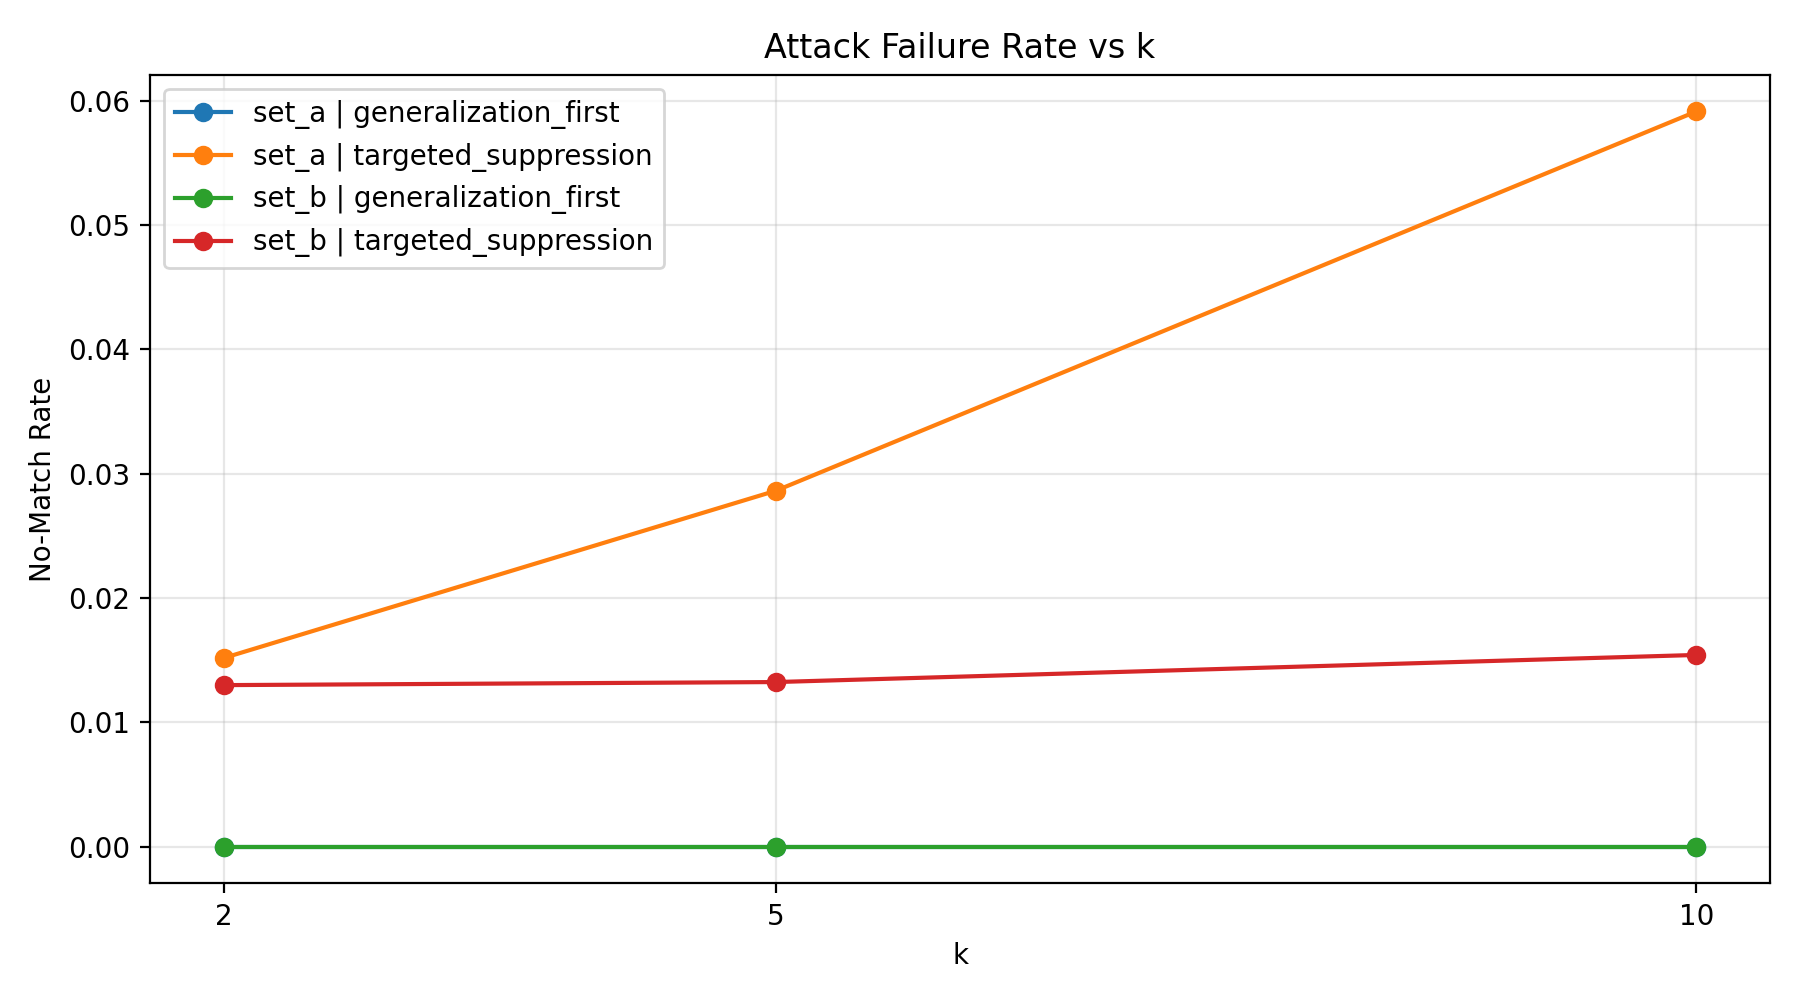
\includegraphics[width=0.88\textwidth]{risk_vs_k.png}
\caption{Attack failure rate (no-match rate) versus $k$. Metrics are averaged across five auxiliary samples.}
\label{fig:risk}
\end{figure}

\subsection{Utility Loss}
Figure~\ref{fig:utility} plots the information-loss score. This metric is more accurate than simple distribution shift because it captures both removed rows and coarse generalization. Under this measure, the difference between the two strategies becomes much clearer: generalization-first has much higher loss even though it preserves row count, while targeted suppression remains far lower across all tested $k$ values.

\begin{figure}[H]
\centering
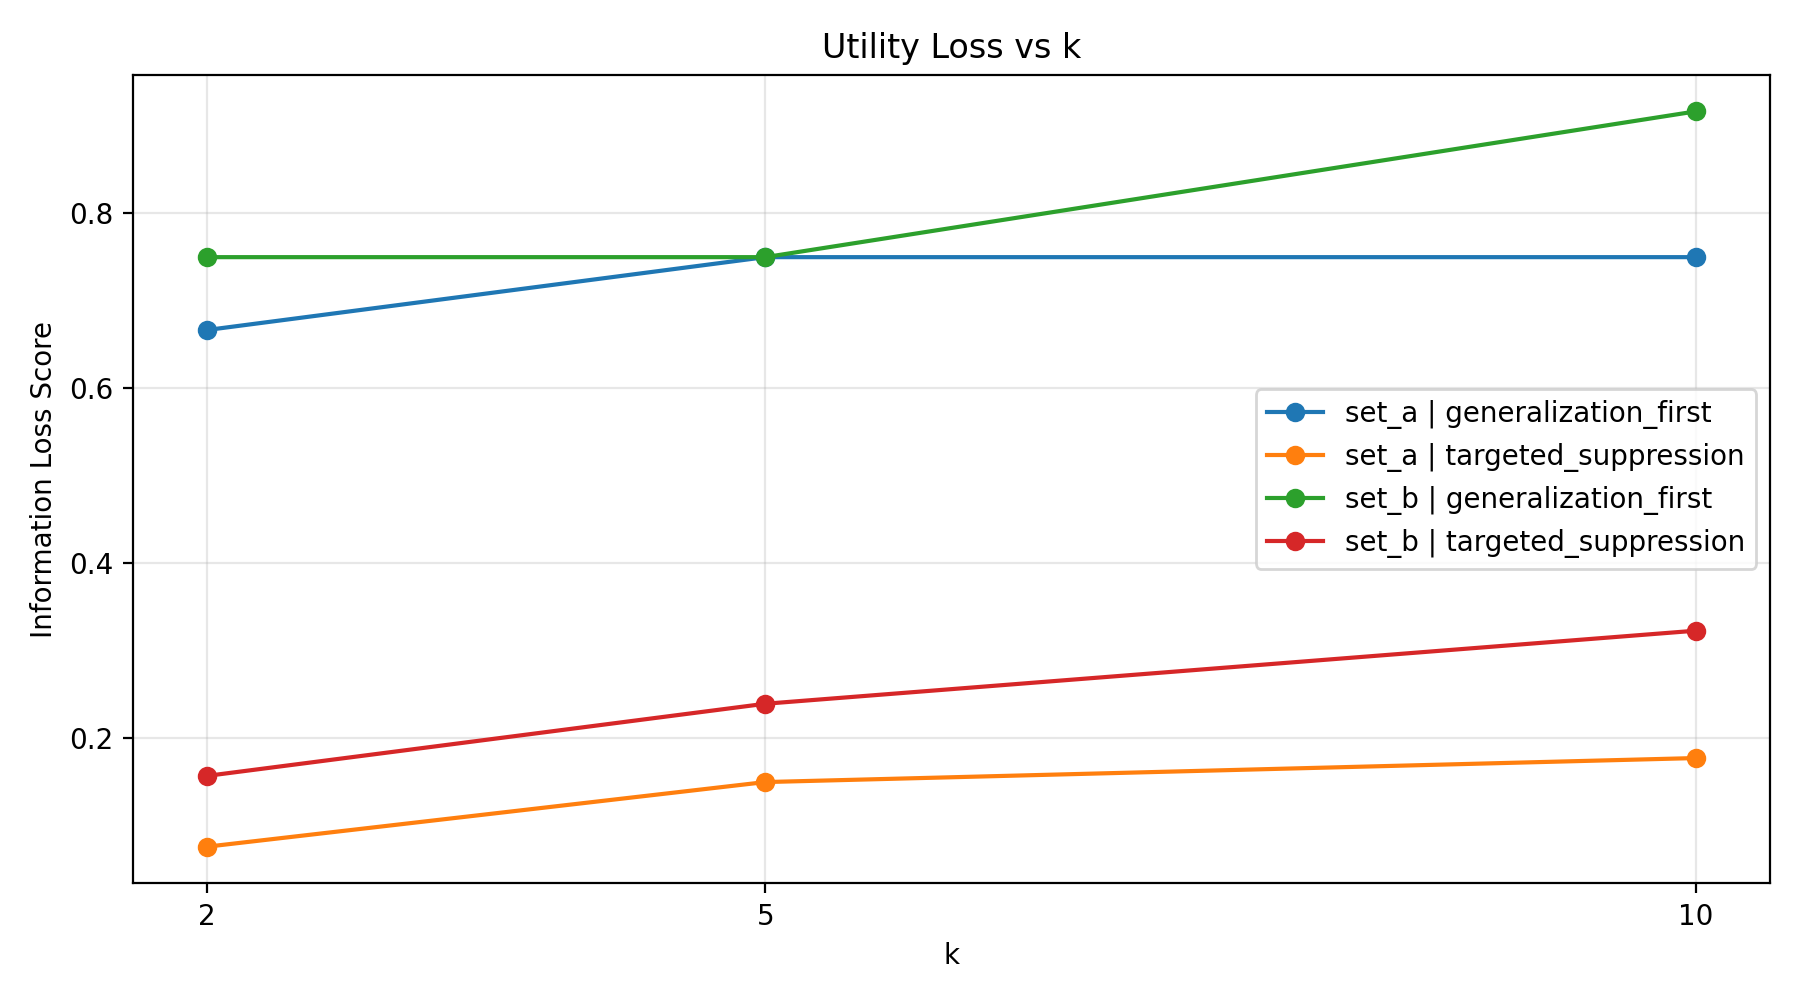
\includegraphics[width=0.88\textwidth]{utility_vs_k.png}
\caption{Utility loss versus $k$, measured by the combined information-loss score.}
\label{fig:utility}
\end{figure}

\subsection{Targeted-Suppression Results}
Table~\ref{tab:targeted_results} summarizes the most practically useful strategy. The improved targeted-suppression pipeline now uses mild generalization to preserve more rows than the earlier baseline while keeping information loss relatively low.

\begin{table}[H]
\centering
\small
\begin{tabular}{llrrrrr}
\toprule
\textbf{QI Set} & \textbf{$k$} & \textbf{Retention} & \textbf{No-Match} & \textbf{Info Loss} & \textbf{Income Shift} & \textbf{Levels} \\
\midrule
Set A & 2 & 98.6\% & 1.5\% & 0.076 & 0.0014 & \texttt{age:1} \\
Set A & 5 & 97.2\% & 2.9\% & 0.150 & 0.0029 & \texttt{age:2} \\
Set A & 10 & 94.0\% & 5.9\% & 0.177 & 0.0065 & \texttt{age:2} \\
Set B & 2 & 98.7\% & 1.3\% & 0.157 & 0.0004 & \texttt{age:1, country:1} \\
Set B & 5 & 98.7\% & 1.3\% & 0.239 & 0.0013 & \texttt{age:1, country:2} \\
Set B & 10 & 98.5\% & 1.5\% & 0.323 & 0.0025 & \texttt{age:1, country:3} \\
\bottomrule
\end{tabular}
\caption{Targeted-suppression results with averaged linkage metrics.}
\label{tab:targeted_results}
\end{table}

Several patterns stand out:
\begin{itemize}[leftmargin=*]
    \item QI Set A at $k=2$ achieves the lowest information loss (0.076) and high retention (98.6\%), making it the best overall balance in this implementation.
    \item QI Set B retains even more rows across all $k$ values, but it does so by progressively generalizing country information, which increases information loss.
    \item For both QI sets, higher $k$ leads to higher attack failure and higher utility loss.
\end{itemize}

\subsection{Generalization-First Results}
Table~\ref{tab:generalization_results} shows why a retention-only view can be misleading. Generalization-first keeps all rows and forces every exact auxiliary match to become ambiguous, but it does so with very large generalization costs.

\begin{table}[H]
\centering
\small
\begin{tabular}{llrrl}
\toprule
\textbf{QI Set} & \textbf{$k$} & \textbf{Retention} & \textbf{Info Loss} & \textbf{Generalization Levels} \\
\midrule
Set A & 2 & 100.0\% & 0.667 & \texttt{age:4, sex:1, education:2, marital\_status:0} \\
Set A & 5 & 100.0\% & 0.750 & \texttt{age:4, sex:1, education:3, marital\_status:0} \\
Set A & 10 & 100.0\% & 0.750 & \texttt{age:4, sex:1, education:3, marital\_status:0} \\
Set B & 2 & 100.0\% & 0.750 & \texttt{age:4, sex:1, occupation:0, native\_country:3} \\
Set B & 5 & 100.0\% & 0.750 & \texttt{age:4, sex:1, occupation:0, native\_country:3} \\
Set B & 10 & 100.0\% & 0.917 & \texttt{age:4, sex:1, occupation:2, native\_country:3} \\
\bottomrule
\end{tabular}
\caption{Generalization-first results.}
\label{tab:generalization_results}
\end{table}

This table captures an important lesson: keeping all rows is not the same as keeping useful detail. The strategy reaches zero unique matches by heavily generalizing age and often suppressing sex or country information completely. That makes the released data much less informative even though simple distribution metrics remain unchanged.

\section{Discussion}
The improved implementation produces a more realistic privacy--utility story than the earlier version.

First, averaging over five auxiliary samples makes the linkage evaluation more stable. Second, allowing mild generalization inside the targeted-suppression strategy reduces unnecessary row loss. Third, the information-loss score makes the utility analysis more honest by penalizing both suppression and coarse generalization.

The results also show that the ``best'' strategy depends on what is valued:
\begin{itemize}[leftmargin=*]
    \item If preserving row count is the only priority, generalization-first looks attractive.
    \item If preserving meaningful detail matters, targeted suppression is clearly better.
    \item If the goal is the most balanced release in this implementation, QI Set A with targeted suppression at $k=2$ is the strongest choice.
\end{itemize}

This final point is important for the seminar project. A privacy method should not be judged only by whether it prevents unique matches. It should also be judged by whether the released data remains interpretable and useful.

\section{Limitations and Ethical Considerations}
This project still has important limitations. It evaluates only k-anonymity, so it does not address attribute disclosure inside homogeneous equivalence classes. The attacker model is simulated from the same source population rather than a truly independent real-world auxiliary database. The utility metrics are stronger than before, but they still do not capture every downstream use of the data.

Nevertheless, the project now provides a more accurate and complete foundation: multiple attack samples, an improved suppression strategy, and a utility measure that reflects both data removal and value coarsening.

Finally, because the dataset contains socially sensitive demographic information, the analysis should be interpreted strictly as a study of anonymization methods, not as a judgment about the represented individuals or groups.

\section{Reproducibility}
The full project can be reproduced from the repository using:
\begin{verbatim}
python3 -m venv .venv
source .venv/bin/activate
python -m pip install -r requirements.txt
python scripts/run_experiments.py
\end{verbatim}

The most relevant files are:
\begin{itemize}[leftmargin=*]
    \item \texttt{data/raw/adult/adult.data}
    \item \texttt{scripts/run\_experiments.py}
    \item \texttt{src/k\_anonymity\_risk\_analysis/*.py}
    \item \texttt{results/metrics/experiment\_summary.csv}
\end{itemize}

\section{Conclusion}
This project implemented and evaluated a complete k-anonymity pipeline for the Adult Census Income dataset. The final version is more accurate and complete than the initial baseline because it averages attack outcomes across multiple auxiliary samples, improves the targeted-suppression strategy with mild generalization, and measures utility with a direct information-loss score.

Across all 12 settings, the exact unique match rate dropped to zero. However, the way that result was achieved mattered greatly. Generalization-first eliminated exact uniqueness by heavily coarsening the released data, while targeted suppression achieved strong privacy with much lower information loss. In this implementation, the best practical trade-off is QI Set A with targeted suppression at $k=2$.

\begin{thebibliography}{9}

\bibitem{SamaratiSweeney1998}
P. Samarati and L. Sweeney.
\newblock Protecting Privacy when Disclosing Information: k-Anonymity and Its Enforcement Through Generalization and Suppression.
\newblock Technical report, SRI International, 1998.

\bibitem{Sweeney2002}
L. Sweeney.
\newblock k-Anonymity: A Model for Protecting Privacy.
\newblock \textit{International Journal of Uncertainty, Fuzziness and Knowledge-Based Systems}, 10(5):557--570, 2002.

\bibitem{BayardoAgrawal2005}
R. J. Bayardo and R. Agrawal.
\newblock Data Privacy through Optimal k-Anonymization.
\newblock In \textit{Proceedings of the 21st International Conference on Data Engineering (ICDE)}, pages 217--228, 2005.

\bibitem{Machanavajjhala2007}
A. Machanavajjhala, J. Gehrke, D. Kifer, and M. Venkitasubramaniam.
\newblock l-Diversity: Privacy Beyond k-Anonymity.
\newblock \textit{ACM Transactions on Knowledge Discovery from Data}, 1(1), 2007.

\bibitem{Li2007}
N. Li, T. Li, and S. Venkatasubramanian.
\newblock t-Closeness: Privacy Beyond k-Anonymity and l-Diversity.
\newblock In \textit{Proceedings of the 23rd International Conference on Data Engineering (ICDE)}, pages 106--115, 2007.

\bibitem{Fung2010}
B. C. M. Fung, K. Wang, R. Chen, and P. S. Yu.
\newblock \textit{Privacy-Preserving Data Publishing: A Survey of Recent Developments}.
\newblock ACM Computing Surveys, 42(4), 2010.

\bibitem{Kohavi1996}
R. Kohavi.
\newblock Scaling Up the Accuracy of Naive-Bayes Classifiers: A Decision-Tree Hybrid.
\newblock In \textit{Proceedings of the Second International Conference on Knowledge Discovery and Data Mining}, 1996.

\bibitem{UCIAdult}
UCI Machine Learning Repository.
\newblock Adult Dataset.
\newblock \url{https://archive.ics.uci.edu/dataset/2/adult}.

\end{thebibliography}

\end{document}
